%!TeX ts-program = xelatex
%!TeX encoding = utf-8 Unicode
\documentclass[ieeetran]{article}
\usepackage{amsmath, amssymb}
\usepackage{graphicx}



\title{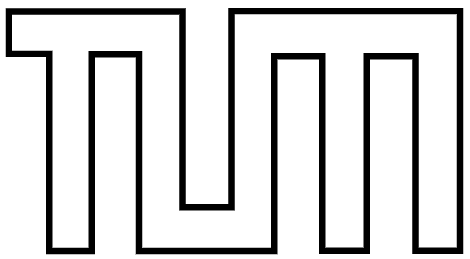
\includegraphics[width=0.43\textwidth]{tumlogo}\hspace{2ex}
\includegraphics[width=0.25\textwidth]{maxlogo}\vspace{1ex}\\ \large \textbf{Max Planck Computing and Data Facility \\Chair of Computer Architecture and Parallel Systems} \vspace{10ex}\\ \huge Efficient Large-Scale Machine Learning with Tensorflow on HPC Systems \vspace{6ex}\\
\large Seminar: Efficient Programming of HPC Systems \\Frameworks and Algorithms\vspace{15ex}}


\author{Efe Kamasoglu}


\begin{document}

\maketitle

\pagebreak

\tableofcontents

\pagebreak

\addcontentsline{toc}{section}{Abstract}

\section*{Abstract}
In the last decade, machine learning has made tremendous progress and become a key technology in many fields. In particular, the size of the real-world data available today have created the need to train models on a large scale. Large-scale machine learning is concerned with the development of algorithms and techniques that allow models to be trained efficiently on huge data sets. As data sets get larger, it is really hard to find a pattern within the data, thus we need to build complexer models in order to make more accurate predictions. High computational power is a necessity when it comes to training complex models. Therefore, we need high performance computing (HPC) systems which are composed of multiple processors and storage units to process the data in parallel. As a result, we can reduce a significant amount of the computation time required for the training of our models. TensorFlow is one the most renowned frameworks to be used in the field of machine learning, which enables us to efficiently program and execute large-scale ML-models on HPC systems. This paper outlines how client programs are efficiently developed with TensorFlow at a large scale and can be run on HPC systems.

\pagebreak

\section{Introduction \& Background} % (fold)
\label{sec:introduction}
TensorFlow is a free and open-source framework developed by Google Brain, which finds its application widely in the field of machine learning and artificial intelligence. It is used to build and train large-scale models according to the client's preferences and provided data sets. In order to train a model, TensorFlow carries out several computations by mapping them onto a variety of hardware, such as mobile devices or systems consisting of multiple computational units with hundreds of GPUs. Those computations are represented in a "directed dataflow graph"\footnote{Martin Abadi, Ashish Agarwal, \ldots, "TensorFlow: Large-Scale Machine Learning on Heterogeneous Distributed Systems," November 9, 2015, p.\ 1, para.\ 2} as a whole, which is then compiled statically or dynamically depending on the version of Tensorflow. 
\\ \\To construct such graph, a client needs to create a session which is an interface with methods of its own. Through those methods, the client can introduce his data set to Tensorflow's system, define his model and its specifications. A graph is typically composed of the following:
\begin{itemize}
  \item \textit{Node:} A node has zero or more inputs and zero or more outputs. It is an instantiation of an operation.
\item \textit{Edge:} Data flows through the edges from one node to another. There are also edges which are not for the dataflow, but for control dependencies between different nodes; e.g., execution order of the concerning operations.
\item \textit{Operation:} An operation represents a computation such as addition or matrix dot product.
\item \textit{Tensor:} Tensors are multidimensional arrays describing the data. They flow into the nodes as inputs through the edges of a graph.
\item \textit{Kernel:} A kernel is an implementation of an operation.
\item \textit{Device:} Devices are computational units on a machine that are utilized by TensorFlow's system to execute kernels. (e.g.\ GPUs)
\end{itemize}
An example graph for a neural network is shown in Figure 1. $W, x$ are tensors which flow into 1.\ node with the operation $MatMul$ as inputs. Matrix multiplication of $W$ and $x$ is then computed and the result as well as tensor $b$ are fed into 2.\ node. Addition of those flow into 3.\ node, where the $ReLU$-function is applied on the addition. In the end, final node is executed, thus cost of the trained model $C$ is computed and returned.
\\ \\Client can either execute all or a part of the graph with the help of the session, where he interacts with the processes that regulate access to devices. In addition to that, TensorFlow system itself has different implementations for execution mechanisms both for single-device and distributed systems.
\begin{figure}[h!]
  \centering
   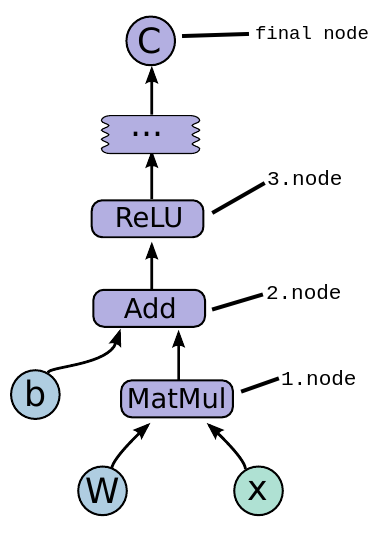
\includegraphics[width=0.25\linewidth]{graph}
\caption[placeholder]{Subgraph example of a neural network for a single neuron}
  \label{fig:graph_caption_placeholder_subgraph_example_for_a_neural_networkfootnotemark}
\end{figure}
\section{Execution of a Graph} % (fold)
\label{sec:execution_of_a_graph}
Each implementation follows the same standard (Fig.\ 2): Firstly, client process calls the master process through the session interface to ignite the execution. An arbitrary number of worker processes, each of which executes a subgraph, are called by the master process. Each worker is responsible for one or more devices. The number of workers depends on the architecture of the system. Master distributes the operations as well as the data tensors to the workers. Also, a worker can fetch the data by itself directly from storage system to the device's memory. Finally, the results are collected by the master and presented to the client process.
\begin{figure}[h!]
  \centering
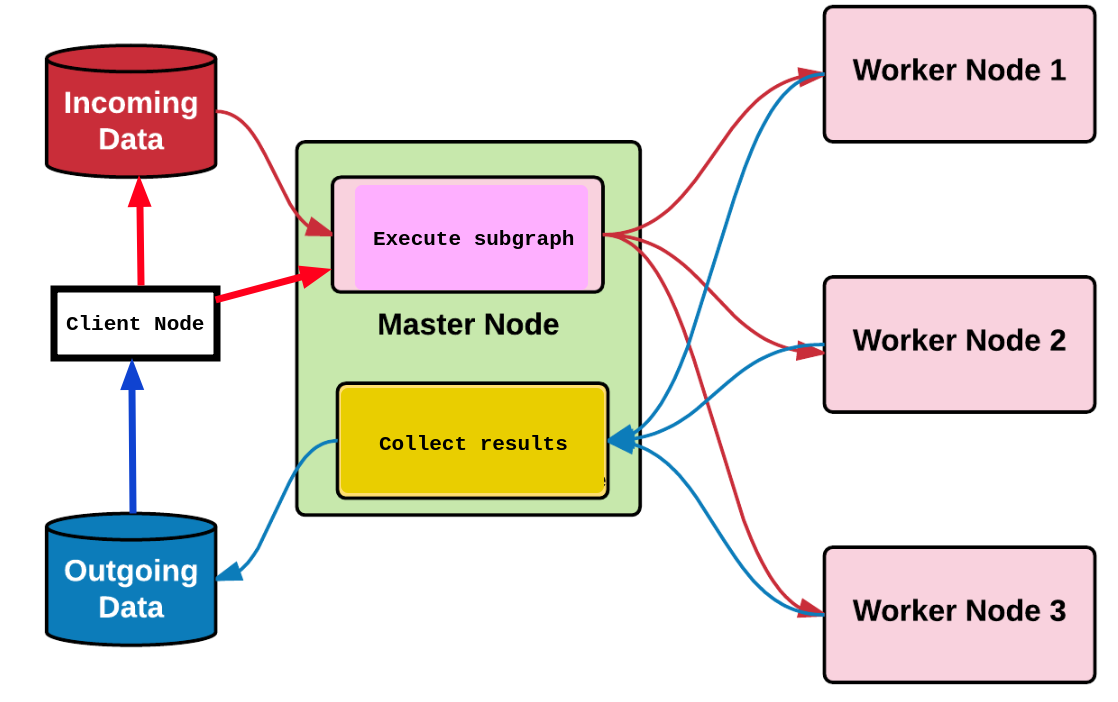
\includegraphics[width=0.5\linewidth]{executionofgraph}
 \caption[placeholder]{Master and Worker processes of a distributed system} 
  \label{fig:executionofgraph}
\end{figure}

\hspace{-0.51cm}A graph can grow immensely due to massive real-world training sets. To ensure efficiency while dealing with such graphs, we need parallelism in terms of task and data. This is why we have to utilize HPC clusters in the first place to save us a huge amount of the computation time.\ As we are going to focus on how to achieve efficiency and scalability while programming with TensorFlow on HPC systems, we first have to take a closer look at the distributed implementation of TensorFlow.


\section{Distributed Implementation of Tensorflow} % (fold)
\label{sec:multiple_device_execution_of_a_graph}
In large-scale machine learning, we have to deal with massive data sets over thousands of petabytes. In order to train a model on such data set and construct a dataflow graph for the model, we need to parallelize our node execution and also divide our data into subsets across multiple devices of our system.
\\ \\If we consider a system with a single device, the execution is fairly simple: A worker process is created for the device. Data is placed into the memory and all the nodes are mapped to the same device. The device executes them in an order according to the control dependencies between the nodes. However, in the case of an HPC system with multiple devices and workers running on different machines, we encounter a handful of programming challenges as to memory management, mapping of the nodes to the different devices and intercommunication between them which includes any type of data transmission (e.g.\ transmitting output of a node to another node as input) required for an operation to be executed.

\subsection{Mapping of the Nodes} % (fold)
\label{sub:mapping_of_nodes} 
TensorFlow uses a greedy algorithm for mapping the nodes: A cost model is prepared by estimating the size of input and output tensors for each node. Graph is traversed according to the dependencies between the nodes. For each node, the execution is simulated with the input tensors on a set of available devices which provide a kernel implementation for the respective operation. Completion time including the time for intercommunication with other devices is either measured or estimated on each device. The results are then gathered and registered on the cost model as well which contains the cost for each particular operation. Finally, the cost model is consulted to make a decision about the mapping. The device with the minimal cost is selected for the operation execution.

\subsection{Intercommunication between Devices} % (fold)
\label{sub:intercommunication_between_devices}
After the node mapping is completed, the full graph is splitted to subgraphs where each subgraph is assigned to a particular device. Due to the structure of the graph, there exist edges between the nodes which are assigned to different devices. Those edges indicate an intercommunication between the concerning devices. To handle the intercommunication efficiently, TensorFlow implements two types of nodes which are only responsible for managing the data transfer from one particular device to another at runtime (in Fig.\ 3): Send-Node and Receive-Node. An edge between the devices ($x \rightarrow y$) is replaced by two edges, one from the node to Send-Node ($x \rightarrow send$) and one from Receive-Node to the other node ($recv \rightarrow y$).
\pagebreak
\begin{figure}[h!]
  \centering
  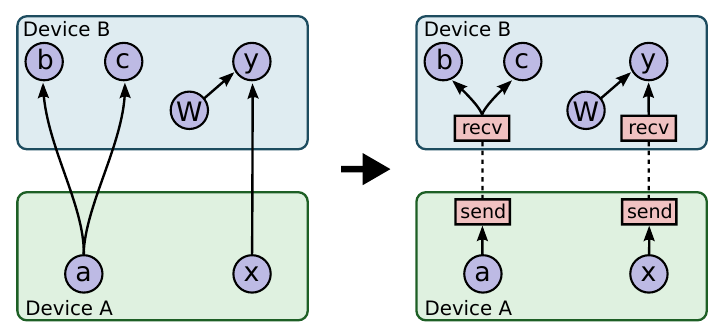
\includegraphics[width=0.5\linewidth]{intercommunication}
  \caption{Replacement of an edge through Send- and Receive-Node}
  \label{fig:intercommunication}
\end{figure}

\hspace{-0.52cm}This way, synchronization of workers (workers for $Device \ A$ and $Device\ B$) is merely delegated to Send- and Receive-Node, where the scheduling and monitoring of intercommunication becomes decentralized across the workers. Therefore, there is no need for the master to coordinate the scheduling of every single node, which directly contributes to scalability.

\subsection{Memory Management} % (fold)
\label{sub:memory_management}
As crucial as performance is, so is memory usage. In scalable machine learning, our aim is to minimize the computation time as well as to optimize the memory management, so that we get most of the job done in a small amount of time without wasting too much memory. When it comes to HPC systems, there are mainly two models which are different architectural approaches as to memory management: shared memory model and distributed memory model.

\subsubsection{Shared Memory Model} % (fold) 
\label{ssub:shared_memory_model}
In a shared memory model, all the worker processes of different devices have access to a common memory, where each worker can modify the data within the shared region as if it is its own address space (in Fig.\ 4). Workers can intercommunicate with each other through the shared memory without the need of an explicit communication nor message passing. The only thing we would need is a method of synchronization to avoid the memory contention. As a result, the latency for intercommunication is constant for each single device, which is an efficient way to process and access the data. Since we do not need any explicit mechanism, implementing the shared memory model is not a complex task, which yields the opportunity to easily program and debug on such system. 
\\ \\However, there are some drawbacks as to the shared memory model in terms of memory capacity, synchronization and scalability. As our machine learning model scales up, it becomes more and more computationally intensive which leads to a significant increase in the number of devices. Thus, the overhead for synchronizing those devices as well as the required capacity would be much higher. This is why we rather prefer a distributed memory model as an efficient solution in the case of larger ML-applications.


\begin{figure}[h!]
  \centering
  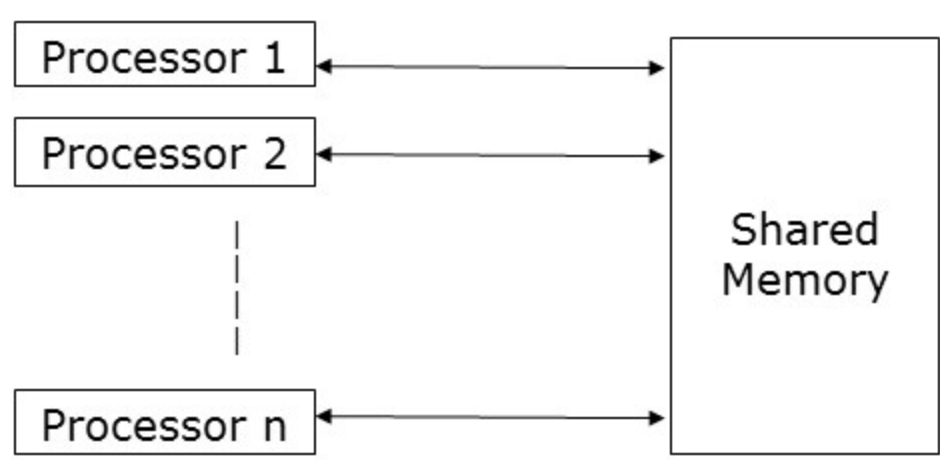
\includegraphics[width=0.4\linewidth]{sharedmemorymodel}
  \caption{Structure of a shared memory model}
  \label{fig:sharedmemorymodel}
\end{figure}


\subsubsection{Distributed Memory Model} % (fold)
\label{ssub:distributed_memory_model}
In a distributed memory model, each device has its own local memory and can directly access only this memory (Fig.\ 5). Data is exchanged between the different workers through a communication network. If a worker wants to access the data of another worker, it uses an explicit communication mechanism such as message passing or remote procedure call. Therefore, we must explicitly implement the intercommunication and coordination between the workers, which is one of the programming challenges, as it adds a significant amount of structural complexity to the system in comparison to the shared memory model. 

\begin{figure}[h!]
  \centering
  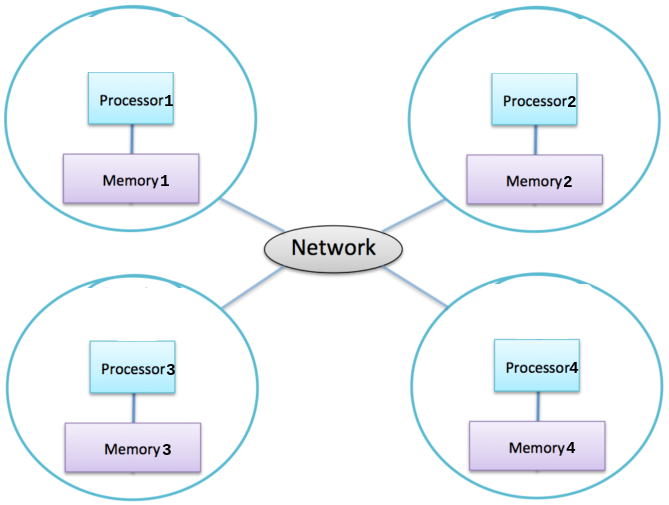
\includegraphics[width=0.4\linewidth]{distributedmemorymodel}
  \caption{Structure of a distributed memory model}
  \label{fig:distributedmemorymodel}
\end{figure}

\hspace{-0.52cm}Despite the complexity of the architecture, distributing memory across multiple devices ensures failure tolerance to great extent. If one cluster malfunctions and is unavailable, other clusters in the network can continue executing because they have their own local memories. We can also be much more flexible on a distributed memory system when it comes to assigning tasks to the workers. Each worker can operate independently and access its own data without relying on others. This gives us the freedom to execute different tasks in parallel and asynchronously.
\\ \\Even though most of the HPC systems have the characteristics of those two memory models combined, the structure of the architecture depends heavily on the use case. For instance, it might be feasible to use a shared memory model in the case of a relatively small convolutional neural network, where we have to constantly compute new gradients in the backpropagation phase and update weights accordingly. By sharing weights and gradients across a common memory region, workers can collaborate efficiently to speed up the training. However, to develop a random forest with a training set of billions of samples, we have to resort to the distributed memory model, as we can parallelize the creation of a batch of decision trees by splitting the training data to our network of workers. Luckily, TensorFlow supports both of the memory models to be as efficient as possible in the creation and execution of a preferred ML-application defined by the client. 
\\ \\Concepts mentioned above are not the only optimization techniques for efficiency and scalability. There are also a lot more provided by TensorFlow itself. Aside from that, a client can exploit TensorFlow's system by using external frameworks for further optimization. 


\section{Optimizations within TensorFlow} % (fold)
\label{sec:optimizations_tensorflow}
In this chapter, we are going to go through some of the optimizations embedded in the implementation of TensorFlow.\ Those optimizations are developed to enhance performance and memory management while taking the extra programming effort off the developer's shoulders at the same time. Some of those optimizations are available in both versions of Tensorflow, whereas the others are only exclusive for Tensorflow 2.X.

\subsection{Common Subexpression Elimination} % (fold)
\label{sub:common_subexpression_elimination}
Common Subexpression Elimination is an optimization technique which aims to eliminate recurring operations. When constructing TensorFlow graphs, certain nodes, whose operations produce the same intermediate result (they are generated through a common subexpression), may be created multiple times. This can lead to unnecessary computation effort, especially for large models. The reason for the repeated creation could either be the client program itself or the specifications of the preferred model.
\\ \\Tensorflow has an algorithm to identify such nodes in the computation graph, where it replaces them with a single node, then redirects the graph. This avoids redundant calculations and improves the efficiency of the execution of the graph.

\subsection{Support for Asynchronous Execution} % (fold)
\label{sub:support_for_asynchronous_kernels}
As we train a model with TensorFlow on an HPC system, its computational graph can be executed mainly in two ways on the multiple devices. If the operations on a number of devices are synchronous, workers of those devices wait for the results of each other before proceeding with the next operation. This execution mode ensures that the operations are executed in a specified fashion according to the control dependencies between the nodes of the graph.
\\ \\Outside of synchronous operations, there are asynchronous ones, as some operations can be executed independently of each other and there is no waiting for the result of other operations. This allows multiple devices to execute unblocked at any time, resulting in potentially better utilization of available resources in some cases (e.g.\ a multi-model ML-application).

\subsection{Eager Execution} % (fold)
\label{sub:eager_execution}
Eager execution refers to a functionality, first introduced in TensorFlow 2, that allows us to perform TensorFlow operations and return the results immediately, thus the computational graph is created dynamically at runtime and executed instantly. In the case of default graph execution in TensorFlow 1, the graph is created beforehand and then executed in a separate step. 
\\ \\Having the eager execution mode on, we could save us the time spent for the graph creation, which speeds up the development process and iteration of the models. It also allows dynamic allocation of the resources during execution. This way, the resources such as devices and memory can be used more efficiently, as they are assigned only for the needed computations.

\subsection{Code Portability} % (fold)
\label{sub:code_portability}
TensorFlow provides features and mechanisms to ensure the code portability across different HPC architectures. One of the features is the support for a variety of operating systems. Moreover, TensorFlow enables developers to write their code independent of the specific hardware through the abstraction of the underlying hardware. Hence, TensorFlow models can run on HPC systems with different devices, CPUs, GPUs or TPUs without having to adapt the code for each specific hardware. TensorFlow also offers compatibility with several HPC-specific libraries such as MPI for distributed communication and CUDA for computation on NVIDIA GPUs.


\section{Optimizations outside of TensorFlow - Horovod} % (fold)
\label{sec:optimization_outside_of_tensorFlow}
Horovod is one of the frameworks by Uber that accelerates the training of large-scale deep learning models on HPC systems by exploiting the distributed implementation of Tensorflow. Motivation for Horovod Project is to develop large-scale ML-applications by utilizing multiple GPUs simultaneously. Fundamental concepts of Horovod are based on the MPI library, which is specifically designed for HPC systems and enables the intercommunication between the worker processes over the network of distributed clusters.
\\ \\As Tensorflow has become an attractive framework for deep learning at Uber, engineering team decided to optimize the training of their models even further. While using the traditional distributed Tensorflow, they have allegedly encountered two major challenges: 1.\ How does the optimal distributed communication structure look like for parameter updates in the model? 2.\ How to reduce the increased complexity of a TensorFlow program, as the model scales?
\\ \\As to the first challenge, they came up with an algorithm called Ring All-reduce for averaging/combining multiple parameters (mostly gradients) of the model computed by several different devices in the network. It is a more efficient way than the common communication algorithm of MPI called All-reduce. This new approach reduces the communication effort and speeds up the training process by, where each device sends data in a ring-like order instead of sending the data to all the other devices.
\\ \\To overcome the second challenge, they simplified the programming by developing a new API that wraps the default TensorFlow API and allows developers to parallelize their models with only a few additional lines of code. This new API also enabled developers to much easily debug and profile their code on a distributed system .

\section{Summary} % (fold)
\label{sec:summary}
As our ML-applications grow, it is almost inevitable to develop them on an HPC system due to the necessity of resources, such as high computational power and enough memory to be able to process a huge data set. TensorFlow provides several handy features to accelerate the development as well as the execution process of such applications, where it delivers solutions in terms of efficient resource management on a distributed system. Those features include algorithms within the implementation of TensorFlow which enable us to effectively distribute task and data over a network of clusters and to let them handle the work in parallel. TensorFlow also provides an intercommunication mechanism between the different clusters, as we need to collect the partial results from our network to build our final model. On top of that, we can decide for a memory management model to get the most out of TensorFlow depending on size and complexity of our desired application. Due to the cross-platform support of Tensorflow, we can write portable code to be run on every piece of hardware. Since we are not only limited to what TensorFlow offers us internally, we can use frameworks like Horovod in conjuction with TensorFlow for further optimization. This way, we delegate some parts of TensorFlow's execution, which we want to optimize, to those frameworks.


\pagebreak
\begin{thebibliography}{3}

\bibitem{first}
Martin Abadi, Ashish Agarwal, Paul Barham, Eugene Brevdo, Zhifeng Chen, Craig Citro, Greg S. Corrado, Andy Davis, Jeffrey Dean, Matthieu Devin, Sanjay Ghemawat, Ian Goodfellow, Andrew Harp, Geoffrey Irving, Michael Isard, Yangqing Jia, Rafal Jozefowicz, Lukasz Kaiser, Manjunath Kudlur, Josh Levenberg,\ldots Xiaoqiang Zheng (November 9, 2015): TensorFlow: Large-Scale Machine Learning on Heterogeneous Distributed Systems 

\bibitem{second}
Yugesh Verma (October 6, 2021): Building Scalable Machine Learning Models with Tensorflow 2.X

\bibitem{third}
How do you choose between shared memory and distributed memory systems for your HPC needs?,\ Retrieved from https://www.linkedin.com/advice/0/how-do-you-choose-between-shared-memory 

\bibitem{fourth}
Orhan G. Yalçın (October 23, 2020): Eager Execution vs.\ Graph Execution in TensorFlow: Which is Better? 

\bibitem{fifth}
Essential documentation, Retrieved from https://www.tensorflow.org/guide 

\bibitem{sixth}
Horovod documentation, Retrieved from https://horovod.readthedocs.io/

\bibitem{seventh}
Alex Sergeev, Mike Del Balso (October 17, 2017): Meet Horovod: Uber’s Open Source Distributed Deep Learning Framework for TensorFlow
\end{thebibliography}





\end{document}
